\tracingstats=0
\iffalse\documentclass{article}\fi
\documentclass[12pt]{article}

\usepackage{sbc-template}
\usepackage{graphicx,url}
\usepackage{verbatim}

%sudo apt install texlive-lang-portuguese
\usepackage[portuguese]{babel}   
\usepackage[utf8]{inputenc} 
%\usepackage{subfigure}
\usepackage{multirow}
\usepackage{graphicx}

\usepackage{algorithm}
\usepackage{algorithmicx}
\usepackage{algpseudocode}

\graphicspath{ {./images/} } 

\sloppy

\title{Avaliação de superpixels para segmentação e detecção de contorno de imagens}

%Avaliar se superpixels podem ser utilizadas na segmentação de imagens sem diminuição do desempenho da segmentação, porém com custo inferior.

\author{Felipe Augusto Lima Reis\inst{1}}

\address{PUC Minas - Pontifícia Universidade Católica de Minas Gerais
  \email{falreis@sga.pucminas.br} }

\begin{document} 

\maketitle

\begin{abstract}
  Superpixels are structures that group similar pixels into sets that reflect aspects of the image. This paper evaluates the use of SLIC and EGB superpixels for segmentation. It's also evaluates the combination of both methods. Finally, this paper shows an hierarchical method implementation, using SLINK (single-linkage) clusterization, applied for the superpixels methods. For evaluation, this paper uses the Berkeley Segmentation Data Set (BSDS500). The results were compared to the dataset ground truth, using precision and recall.
\end{abstract}
     
\begin{resumo} 
  Superpixels são estruturas que agrupam pixels semelhantes em conjuntos que refletem aspectos da imagem. Este artigo avalia a utilização de superpixels SLIC e EGB para segmentação. Avalia também os benefícios da combinação dos métodos para produção de segmentação. Por fim, o artigo mostra uma implementação de método hierárquico, utilizando clusterização SLINK (\textit{single-linkage}), para os métodos estudados nesse trabalho. Para avaliação dos resultados, foram utilizadas as imagens do conjunto de validação do Berkeley Segmentation Data Set (BSDS500). Os resultados foram com comparadas em relação ao \textit{ground truth}, utilizando o método de precisão e revocação.
\end{resumo}


\section{Introdução} \label{sec:introducao}

A segmentação consiste em dividir uma imagem em um conjunto de regiões logicamente agrupadas, de modo a reunir áreas que contêm informação relevante dentro dos grupos, idealmente correspondente a objetos reais \cite{DOMINGUEZ} \cite{ZHANG2008}. A segmentação é utilizada no processamento de imagens, vídeos e aplicações de visão computacional. Consiste, ainda, em um importante passo na tentativa de explicar uma imagem por meio de algoritmos \cite{ZHANG2008}. Extensiva pesquisa é realizada e muitas abordagens e algoritmos são utilizados, com bons resultados para um conjunto ou classes de imagens \cite{ZHANG2008}. 

Para tarefas de segmentação, os \textit{pixels} podem ser tomados como unidades básicas de processamento \cite{WANG201728}. O agrupamento de pixels em unidades maiores permite um tipo de segmentação chamado de \textit{oversegmentation} \cite{WANG201728}, ilustrado na Figura \ref{fig:superpixel}. Alguns métodos de geração de superpixels são utilizados para segmentação de imagens e detecção de bordas, como os métodos EGB \cite{FELZENSZWALB} e SLIC \cite{SLIC}. Esse trabalho analisa a utilização de métodos de segmentação e detecção de contornos baseados em superpixels. Também analisa o agrupamento de superpixels e a criação de hierarquias, permitindo maior ou menor nível de detalhamento para uma representação.

\begin{figure}[ht]
\centering
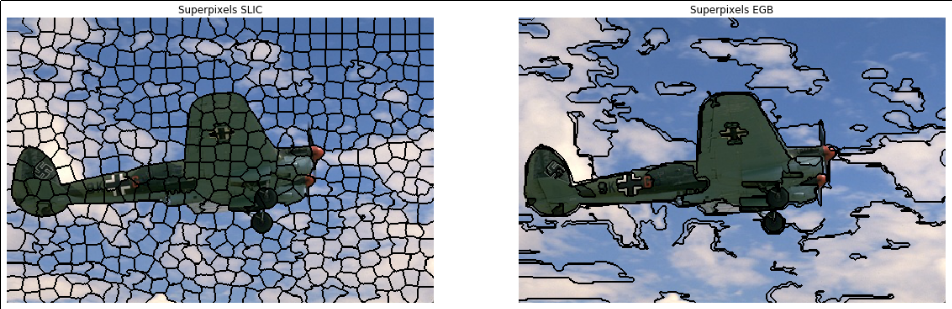
\includegraphics[width=1.\textwidth]{superpixels.png}
\caption{Imagens segmentadas utilizando superpixels SLICO e EGB}
\label{fig:superpixel}
\end{figure}

O presente trabalho apresenta a seguinte estrutura: a Seção \ref{sec:ref_teorico} mostra o referencial teórico para construção do trabalho, a Seção \ref{sec:mat_metodos}, exibe os métodos desenvolvidos, algoritmos e os critérios para elaboração dos testes; a Seção \ref{sec:testes} mostra os resultados obtidos nos testes realizados e a discussões dos mesmos; a Seção \ref{sec:conclusao} contém a conclusão do artigo, com as considerações finais.

%%%%%%%%%%%%%%%%%%%%%%%%%%%%%%%%%%%%%%%%%%%%%%%%%%%%%%%
%%%%%%%%%%%%%%%%%%%%%%%%%%%%%%%%%%%%%%%%%%%%%%%%%%%%%%%
%%%%%%%%%%%%%%%%%%%%%%%%%%%%%%%%%%%%%%%%%%%%%%%%%%%%%%%


\section{Referencial Teórico} \label{sec:ref_teorico}

%%%%%%%%%%%%%%%%%%%%%%%%%%%%%%%%%%%%%%%%%%%%%%%%%%%%%%%
%%%%%%%%%%%%%%%%%%%%%%%%%%%%%%%%%%%%%%%%%%%%%%%%%%%%%%%

\subsection{Superpixels} \label{ssec:super}

Superpixels são estruturas que agrupam pixels semelhantes em conjuntos. O agrupamento possibilita a redução de complexidade das tarefas de processamento \cite{SLIC}, ao reduzir a quantidade de itens a serem processados. Os superpixels são utilizados na área de visão computacional para solução de vasto número de problemas, como detecção de contorno \cite{CONTOUR}, segmentação \cite{SEG_MERGE} e localização de objetos \cite{SEG_LOCALIZ}.

Superpixels, segundo \cite{FELZENSZWALB}, devem capturar importante grupos ou regiões, refletindo aspectos da imagem. Devem também ser executados em tempo próximo ao linear em relação a quantidade de pixels. Existem diversas abordagens para a geração de superpixels, que podem ser classificadas, segundo o método de agrupamento, em dois grandes grupos \cite{SLIC}: 

\begin{itemize}
 \item \textit{Algoritmos baseados em grafos}: tratam cada pixel como um nó do grafo. Os pesos das arestas são proporcionais a similaridade entre os pixels vizinhos \cite{SLIC}. Dentre os algoritmos baseados em grafos podemos citar o \textit{Efficient Graph-Based Image Segmentation} (EGB) \cite{FELZENSZWALB};
 \item \textit{Algoritmos baseados em gradiente ascendente}: partem de um conjunto inicial de pixels e utilizam métodos de gradiente ascendente iterativamente para refinar os conjuntos (\textit{clusters}) até que se atinja um critério de convergência \cite{SLIC}. Nesse conjunto, podemos  citar as abordagens \textit{watersheds} \cite{WATERSHEDS} e o algortimo SLIC (\textit{Simple Linear Iteravite Clustering}) \cite{SLIC}
\end{itemize}

%%%%%%%%%%%%%%%%%%%%%%%%%%%%%%%%%%%%%%%%%%%%%%%%%%%%%%%

\subsubsection{Superpixels SLIC e SLICO} \label{sssec:slic}

O algoritmo SLIC utiliza um único parâmetro $k$, correspondente a quantidade aproximada de superpixels, gerados em formato regular \cite{SLIC}. A Figura \ref{fig:SLICO} ilustra o algoritmo SLIC para diferentes números de superpixels. A fim de produzir tamanhos semelhantes, o intervalo de busca analisado é \mbox{$S=\sqrt{N/k}$}, onde $N$ é o número de pixels da imagem \cite{SLIC}. 

A definição do centro dos superpixels é feita utilizando sementes, que são movidas para locais de geração. Esses locais corresponem a posição mais baixa do gradiente em uma vizinhança de 3x3 \cite{SLIC}. Esse passo evita que superpixels sejam centrados nas bordas ou em um posição de ruído \cite{SLIC}. Cada pixel, então, é associado com o centro do cluster mais próximo, de modo que as regiões de busca se sobreponham \cite{SLIC}. A fim de aumentar o desempenho do algoritmo, a região de busca é limitada em 2 vezes o tamanho aproximado do superpixel $S$, gerando busca em uma área $2S \times 2S$ \cite{SLIC}. Em seguida, um passo atualiza os centros dos clusters e computa o erro residual $E$ \cite{SLIC}. O Algoritmo \ref{alg:SLIC}, resume as informações descritas nesse parágrafo.

\begin{algorithm}
    \caption{Segmentação por superpixels SLIC (\textit{Adaptado de } \cite{SLIC})}
    \label{alg:SLIC}
    \begin{algorithmic}[1]
        \State{\textit{ /* Inicialização */}}
        \State{Inicialize os centros dos clusters $C_k = [l_k, a_k, b_k, x_k, y_k]^T$ por amostragem de pixels em etapas de grade regulares $S$}
        \State{Mova os centros dos clusters para a posição de menor gradiente em uma vizinhança $3 \times 3$}
        \State{Faça label $l(i) = -1$ para cada pixel $i$}
        \State{Faça distância $d(i) = \infty $ para cada pixel $i$}
        \Repeat
            \For{cada cluster centrado em $C_k$}
                \For{cada pixel $i$ em uma região $2S \times 2S$ ao redor de $C_k$}
                \State{Compute a distância $D$ entre $C_k$ e $i$}
                \If{$D < d(i)$}
                    \State{faça $d(i) = D$}
                    \State{faça $l(i) = k$}
                \EndIf
                \EndFor
            \EndFor    
            \State{\textit{ /* Atualização */}}
            \State{Compute novos centros dos clusters}
            \State{Compute o erro residual $E$}
        \Until{$E \leq threshold$}
    \end{algorithmic}
\end{algorithm}


Para compreensão mais precisa do Algoritmo \ref{alg:SLIC}, é necessário entender o método para cálculo da medida de distância $D$ entre os conjuntos. O algoritmo SLIC trabalha no espaço de cores $CIELAB$ junto ao espaço-plano $labxy$ \cite{SLIC}. Nesse cenário, a posição do pixel pode assumir um intervalo de valores, fazendo com que o cálculo da distância não possa ser feito utilizando uma distância euclidiana; é necessária uma prévia normalização da proximidade espacial e da cor \cite{SLIC}. 

No espaço de cores $CIELAB$, cada pixel de cores é representado por $[l a b]^T$, sendo que uma grande variedade de valores é possível \cite{SLIC}. A posição do pixel $[x y]^T$, por sua vez, pode asssumir um conjunto de valores de acordo com o tamanho da imagem \cite{SLIC}. A definição simples de $D$ como uma distância Euclidiana de 5 dimensões no espaço $labxy$, pode causar inconsistências no comportamento dos clusters para diferentes tamanhos de superpixels \cite{SLIC}. Em superpixels grandes, as distâncias espaciais superam a proximidade da cor, dando mais importância relativa à proximidade espacial do que à cor \cite{SLIC}, fazendo com que os superpixels não sejam aderentes as bordas. Para solucionar o problema, é necessário normalizar a proximidade espacial ($S$) e de cores ($C$), com as respectivas distâncias máximas dentro do cluster $N_s$ e $N_c$. Com isso, considerando $d_c = \sqrt{(l_j - l_i)^2 + (a_j - a_i)^2 + (b_j - b_i)^2}$ a distância entre as cores e $d_s =  \sqrt{(x_j - x_i)^2 + (y_j - y_i)^2}$, a distância espacial, temos:

\begin{equation}
 D' = \sqrt{ \left(\frac{d_c}{N_c} \right)^2 + \left(\frac{d_s}{N_s} \right)^2}
 \label{equ:CIELAB1}
\end{equation}

Como a distância espacial máxima esperada dentro de um cluster corresponde ao tamanho da amostra $N_S = S = \sqrt{N/K}$, e considerando também que a distância máxima de cores $N_c$, pode variar de cluster para cluster, podemos fixar $N_c$, como uma constante $m$ e reescrever a Equação \ref{equ:CIELAB1} \cite{SLIC}:

\begin{equation}
 D' = \sqrt{ \left(\frac{d_c}{m} \right)^2 + \left(\frac{d_s}{S} \right)^2}
 \label{equ:CIELAB2}
\end{equation}

A Equação \ref{equ:CIELAB2}, por sua vez, pode ser simplificada na forma adotada pelos autores, como na Equação \ref{equ:CIELAB3} \cite{SLIC}:

\begin{equation}
 D = \sqrt{d_c^2 + \left(\frac{d_s}{S} \right)^2 \cdot m^2}
 \label{equ:CIELAB3}
\end{equation}

Uma etapa extra no processo de pós-processamento é a união de \textit{pixels orfãos}. Esses pixels são adicionados ao cluster mais próximo usando o algoritmo de componentes conexos \cite{SLIC}.

A complexidade do algoritmo SLIC é $O(n)$, devido a limitação do espaço de pesquisa do algoritmo SLIC \cite{SLIC1}. Outros algoritmos que utilizam \textit{k-means} para segmentação tem custo $O(kNI)$, onde $N$ é o número de pontos (\textit{pixels} na imagem), $k$ corresponde ao número de clusters (ou sementes) e $I$ corresponde ao número de iterações para convergência \cite{SLIC1}. A modificação no algoritmo SLIC está na redução de cálculos redundantes de distância \cite{SLIC1}. 

\begin{figure}[ht]
\centering
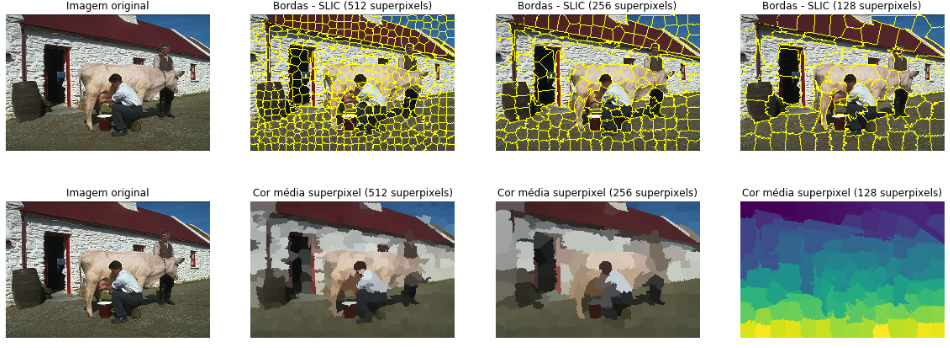
\includegraphics[width=1.\textwidth]{slic_segmentation_compare.png}
\caption{Fronteiras e coloração pelo valor médio dos superpixels SLIC/SLICO, para diferentes quantidades de superpixels}
\label{fig:SLICO}
\end{figure}

%%%%%%%%%%%%%%%%%%%%%%%%%%%%%%%%%%%%%%%%%%%%%%%%%%%%%%%

\subsubsection{Superpixels EGB} \label{sssec:egb}

Os superpixels EGB (\textit{Efficient Graph-Based Image Segmentation}), demonstrados na Figura \ref{fig:EGB}, utilizam uma abordagem baseada em grafos não direcionados. Nela, cada \textit{pixel} corresponde a um nó do grafo e a ligação entre eles ocorre por meio de arestas, com pesos não negativos, correspondente a medida de dissimilaridade \cite{FELZENSZWALB}. 

A segmentação $S$ é uma partição dos vértices $V$ em componentes, no qual cada região $C \in S$ corresponde a um componente conectado a um grafo $G'=(V,E')$, onde $E' \subseteq E$, ou seja, a segmentação é induzida por um conjuntos de vértices em arestas $E$ \cite{FELZENSZWALB}.

No algoritmo proposto por \cite{FELZENSZWALB} foi definido um predicado $D$ para avaliação da evidência de bordas entre dois componentes de uma segmentação. São avaliadas as dissimilaridades entre elementos de dois componentes e comparados a elementos vizinhos, de modo que o algoritmo possa se adaptar em relação as características dos dados \cite{FELZENSZWALB}. 

Para a comparação entre as regiões é utilizada uma função de corte (\textit{threshold}) $\tau$, a fim de medir o grau de dissimilaridade, que deve ser superior a diferença interna mínima, evidenciando uma borda \cite{FELZENSZWALB}. A função de corte, no algoritmo, é baseada no tamanho do componente $\tau=k/|C|$, onde $|C|$ corresponde ao tamanho do componente $C$ e $k$ corresponde a um parâmetro do algoritmo \cite{FELZENSZWALB}.

O algoritmo EGB, utilizando pesos inteiros e ordenação por contagem, pode ser executado com custo linear e com complexidade $O(nlogn)$, para qualquer método de ordenação \cite{FELZENSZWALB}. 

\begin{figure}[ht]
\centering
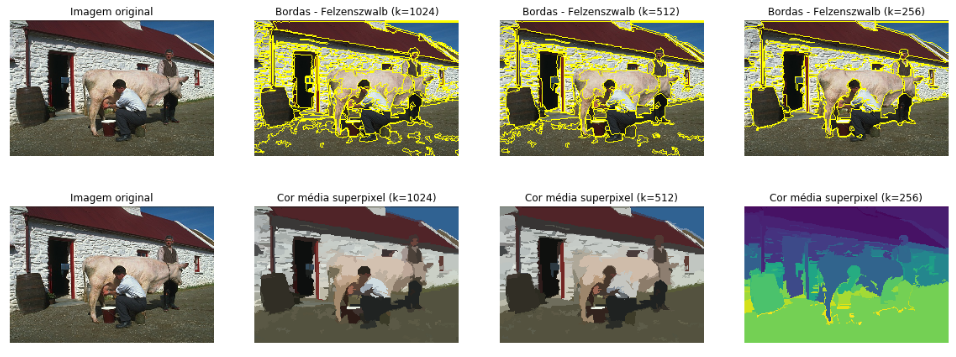
\includegraphics[width=1.\textwidth]{felz_segmentation_compare.png}
\caption{Fronteiras e coloração pelo valor médio dos superpixels EGB, para diferentes quantidades de superpixels}
\label{fig:EGB}
\end{figure}

%%%%%%%%%%%%%%%%%%%%%%%%%%%%%%%%%%%%%%%%%%%%%%%%%%%%%%%
%%%%%%%%%%%%%%%%%%%%%%%%%%%%%%%%%%%%%%%%%%%%%%%%%%%%%%%

\subsection{Análise de Clusters} \label{ssec:clusters}

Análise de cluster é a tarefa de agrupar dados em grupos (\textit{clusters}) que tenham características em comum, de modo que sejam signinficativos e/ou úteis \cite{CLUSTER_HIER}. \textit{Clusters} hierárquicos correspondem a análise de \textit{clusters} com finalidade de buscar hierarquias entre eles. As estratégias para hierarquização de cluster se dividem em dois grupos \cite{ROKACH}:

\begin{itemize}
 \item Aglomerativo - abordagem \textit{``bottom up''}, em que a observação inicia-se no próprio \textit{cluster} e os pares de \textit{clusters} são unidos na medida em que se sobe na hierarquia. 
 \item Divisivo - abordagem \textit{``top down''} onde as observações iniciam-se em um \textit{cluster} e são realizados agrupamentos recursivos a medida em que se desce na hierarquia.
\end{itemize}

Os algoritmos de clusterização hierárquicos aglomerativos podem ser classificados, em geral, como gulosos \cite{SINGLE_LINKAGE}. Uma sequência de passos irreversíveis são tomados para construção dos dados desejados \cite{SINGLE_LINKAGE}. A abordagem de \textit{clustering} hierárquico de ligação única (\textit{single-linkage}) produz um conjunto de \textit{clusters} em cada nível - ou para cada valor-limite que produz uma nova partição \cite{SINGLE_LINKAGE}. O nome ligação única surge quando a dissimilaridade de interconexão entre dois grupos (ou componentes) é definida como a menor diferença de interconexão entre um membro de um e um membro do outro grupo \cite{SINGLE_LINKAGE}.

Os algoritmos originais de clusterização possuem complexidade $O(n^3)$. Alguns algoritmos de \textit{single-linkage}, entretanto, como o SLINK, possuem complexidade $O(n^2)$ \cite{SLINK} \cite{SINGLE_LINKAGE}. O SLINK utiliza a distância mínima como critério de ligação (\textit{linkage}) entre os \textit{clusters}. A fórmula de dissimilaridade de Lance-Williams $min\{d_{ik}, d_{jk}\}$, corresponde a distância mínima para dois pares de clusters $i$ e $j$ observados, onde $d$ é a métrica de distância escolhida \cite{SINGLE_LINKAGE}.

A partir da aglomeração de \textit{clusters} é possivel construir uma árvore hierarquica binária, onde os clusters são agrupados por sua similaridade. Esse tipo de árvore binária para visualização também é conhecido como dendrograma \cite{SINGLE_LINKAGE}.

%%%%%%%%%%%%%%%%%%%%%%%%%%%%%%%%%%%%%%%%%%%%%%%%%%%%%%%
%%%%%%%%%%%%%%%%%%%%%%%%%%%%%%%%%%%%%%%%%%%%%%%%%%%%%%%

\subsection{Precisão e Revocação} \label{ssec:prec_recall}

Nos problemas de decisão os classificadores podem ser positivos ou negativos \cite{PRECISION_RECALL}. A decisão feita por um classificador pode ser representada por uma estrutura conhecida como matriz de confusão ou tabela de contigência. Essa matriz pode identificar 4 tipos de dados possíveis \cite{PRECISION_RECALL}:

\begin{itemize}
 \item Verdadeiros Positivos - correspondem aos valores que foram corretamente classificados como positivos;
 \item Falsos Negativos - correspondem aos valores que foram classificados incorretamente como negativos;
 \item Falsos Positivos - correspondem aos valores que foram classificados incorretamente como positivos;
 \item Verdadeiros Negativos - correspondem aos valores que foram classificados corretamente como negativos \cite{PRECISION_RECALL};
\end{itemize}

O método de precisão e revocação é um método de classificação binária, onde a precisão (\textit{prediction}) mede a proporção de eventos do modelo que são reais; enquanto a revocação (\textit{recall}), mede a proporção de eventos ocorridos no domínio que são capturados pelos modelos \cite{PREC_RECALL_REGR}. 

A partir dos valores de precisão e revocação, é possível construir curvas que associem ambos os valores. Essas curvas possibilitam uma informação visual da performance de um algoritmo \cite{PRECISION_RECALL}. Outra classificação pode ser dada por uma média harmônica, chamada de \textit{F-measure} \cite{F_MEASURE}. Essa medida é utilizada para diferentes problemas de classificação e impõe um melhor equilíbrio entre precisão e revocação, respectivamente, e, portanto, é mais adequado no caso de dados desequilibrados \cite{F_MEASURE}. 

Dado um vetor binário $m$-dimensional e classes de precisão e revocação, cujo conjunto estejam associados ao vetor $m$-dimensional, a medida \textit{F-measure} é dada pela Equação \ref{equ:PREC_RECALL}, correspondente a média harmônica entre ambas as medidas \cite{F_MEASURE}.

\begin{equation}
 F=\frac{ 2 \sum\limits_{i=1}^m {prec \cdot revoc}}{ \sum\limits_{i=1}^m {prec} + \sum\limits_{i=1}^m {revoc}}  \in [0,1]
 \label{equ:PREC_RECALL}
\end{equation}

%%%%%%%%%%%%%%%%%%%%%%%%%%%%%%%%%%%%%%%%%%%%%%%%%%%%%%%
%%%%%%%%%%%%%%%%%%%%%%%%%%%%%%%%%%%%%%%%%%%%%%%%%%%%%%%

\subsection{Hierarquia de Segmentações} \label{ssec:hierarq_segmentacao}

A hierarquização das segmentações tem como objetivo possibilitar a utilização dos algoritmos para agrupar segmentação em diferentes níveis de detalhamento: desde um nível mais aprofundado até o macro. Os diferentes níveis podem ser combinados em termos do contorno das hierárquias, permitindo a representação como bordas suaves, chamadas Mapas de Contorno Ultramétrico (\textit{UCM - Ultrametric Contour Map}) \cite{ULTRAMETRIC}.

Para que os níveis hierárquicos possam garantir a manutenção da informação, agrupando apenas características semelhantes, as hierarquias devem seguir os princípios de análise multiescala \cite{SILVIO_ZENILTON}. Esses princípios asseguram manutenção de duas características principais \cite{SILVIO_ZENILTON}:

\begin{itemize}
 \item Causalidade - um contorno presente em uma escala $k1$ deve estar presente em qualquer escala $k2 < k1$ \cite{SILVIO_ZENILTON};
 \item Localidade - a medida em que o número de regiões diminui, os contornos devem ser estáveis (não devem se mover). A união corresponde a manutenção das bordas dos grupos que se fundiram \cite{SILVIO_ZENILTON}.
\end{itemize}

%%%%%%%%%%%%%%%%%%%%%%%%%%%%%%%%%%%%%%%%%%%%%%%%%%%%%%%
%%%%%%%%%%%%%%%%%%%%%%%%%%%%%%%%%%%%%%%%%%%%%%%%%%%%%%%
%%%%%%%%%%%%%%%%%%%%%%%%%%%%%%%%%%%%%%%%%%%%%%%%%%%%%%%

\section{Métodos} \label{sec:mat_metodos}

Para confecção do trabalho foram escolhidos os algoritmos de SLIC e EGB. Os algoritmos possuem características diferentes: o SLIC é capaz de produzir \textit{superpixels} em formas regulares, porém não é tão preciso ao separar os conjuntos por similaridade; por outro lado, o EGB, produz \textit{superpixels} irregulares, porém é mais aderente às diferenças de cores entre \textit{pixels}.

Nos testes foi executada hierarquização dos resultados obtidos após a geração de superpixels SLIC, EGB e também sobre a composição SLIC+EGB. A composição SLIC+EGB corresponde a aplicação do algoritmo SLIC, seguido pela recoloração utilizando o valor médio de cores do \textit{superpixel} e, por fim, a aplicação do método EGB. A partir dessa seção, a composição dos métodos SLIC e EGB passará a ser chamado, nesse trabalho, de SGB, para facilitar a nomenclatura.

Os resultados das hierarquizações foram comparados aos melhores resultados de segmentação obtidos pela segmentação SLIC, EGB e SGB sem hierarquização. O método de hierarquização está descrito na Seção \ref{ssec:hierquia_segm}. Informações sobre a base de dados utilizada para comparação dos métodos está presente na Seção \ref{ssec:base_dados}, enquanto o método de avaliação de resultados está descrito na Seção \ref{ssec:aval_resultados}. Os resultados dos testes estão disponíveis na Seção \ref{sec:testes}.

%%%%%%%%%%%%%%%%%%%%%%%%%%%%%%%%%%%%%%%%%%%%%%%%%%%%%%%
%%%%%%%%%%%%%%%%%%%%%%%%%%%%%%%%%%%%%%%%%%%%%%%%%%%%%%%

\subsection{Hierarquias} \label{ssec:hierquia_segm}

% %%%%%%%%%%%%%%%%%%%%%%%%%%%%%%%%%%%%%%%%%%%%%%%%%%%%%%%

Para construção das hierarquias foram gerados \textit{clusters} com as correlações entre os grupos de \textit{superpixels} adjcentes, após a segmentação inicial. Foi utilizado o algoritmo SLINK (\textit{single-linkage}) para agrupamento dos \textit{superpixels} próximos, gerando uma árvore com as correlações entre os \textit{superpixels}.

Para verificação da estrutura da árvore foi utilizado um dendrograma, como representado na Figura \ref{fig:DENDROGRAM}. O dendrograma é um tipo de árvore binária utilizado para ilustração de uma clusterização hierarquica \cite{SINGLE_LINKAGE}.

\begin{figure}[ht]
\centering
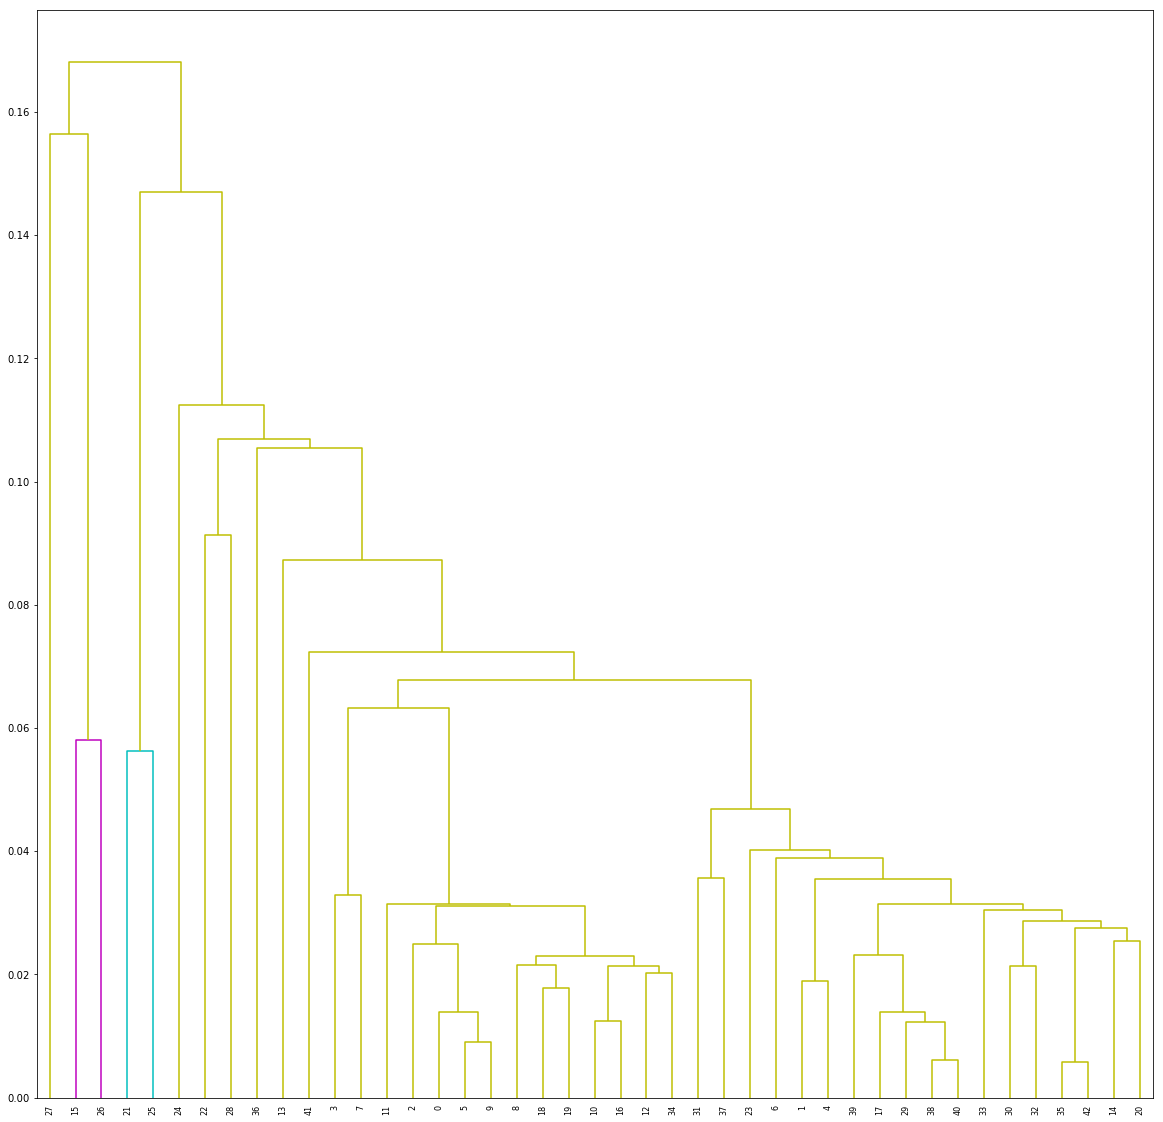
\includegraphics[width=0.9\textwidth]{dendrogram.png}
\caption{Dendrograma dos superpixels de uma imagem}
\label{fig:DENDROGRAM}
\end{figure}

Em um árvore de estrutura semelhante à representada por um dendrograma é possível realizar cortes horizontais ou verticais na hierarquia, a fim de obter tipos de agrupamentos diferentes. Nesse trabalho foram realizados cortes horizontais, em diversos níveis. 

Devido às características da segmentação, quando comparados ao \textit{ground truth}, não foram validados todos os níveis hierárquicos. Com o objetivo de reduzir o número de comparações pelo \textit{benchmark} de classificação de resultados, foram avaliados níveis hierárquicos intermediários que apresentaram melhores resultados em testes empíricos. 

Foi estabelecido um limite máximo e mínimo para os cortes na hierarquia, de modo que os cortes foram realizados dentro de um intervalo, evitando avaliação de níveis com baixa probabilidade de adequação ao \textit{ground truth}. Os cortes foram feitos de forma não sequencial, com espaçamento entre eles, para aumentar, a faixa de possíveis bons resultados, sem, entretanto, produzir inúmeras segmentações diferentes. 

O método de hierarquização descrito nesse trabalho manteve as características da análise multiescala, descritos na Seção \ref{ssec:hierarq_segmentacao}. A Figura \ref{fig:hierarq_partit} mostra os possíveis cortes na hierarquia de uma segmentação SGB, com marcação somente das bordas.

É importante salientar que os métodos SLIC e EGB originais, quando apenas variados os parâmetros de criação de superpixels não mantêm as características de análise multiescala, conforme podemos ver nas Figuras \ref{fig:SLICO} e \ref{fig:EGB}; essas características somente são obtidas pelos processos hierárquicos aplicados aos métodos.

\begin{figure}[ht]
\centering
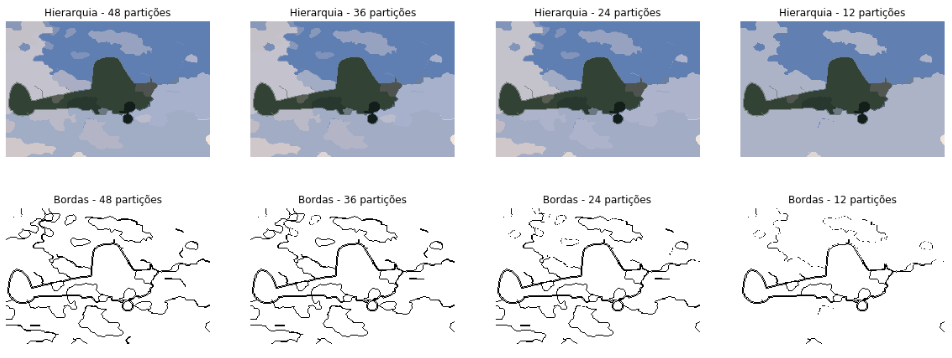
\includegraphics[width=1.\textwidth]{slic_hierarquia_particoes.png}
\caption{Hierarquia de partições utilizando superpixel SLIC+EGB.}
\label{fig:hierarq_partit}
\end{figure}

%%%%%%%%%%%%%%%%%%%%%%%%%%%%%%%%%%%%%%%%%%%%%%%%%%%%%%%
%%%%%%%%%%%%%%%%%%%%%%%%%%%%%%%%%%%%%%%%%%%%%%%%%%%%%%%

\subsection{Base de Dados} \label{ssec:base_dados}

Para avaliação dos algoritmos e suas versões hierárquicas, foi utilizada a base de dados BSDS500 (\textit{Berkeley Segmentation Data Set and Benchmarks 500}). A base BSDS500 provê um conjunto de imagens naturais com suas respectivas segmentações manuais para pesquisa de segmentação e detecção de bordas \cite{BSDS500}. Essa base de dados é uma extensão da BSDS300, com 200 novas imagens para avaliação \cite{BSDS500}.

%%%%%%%%%%%%%%%%%%%%%%%%%%%%%%%%%%%%%%%%%%%%%%%%%%%%%%%
%%%%%%%%%%%%%%%%%%%%%%%%%%%%%%%%%%%%%%%%%%%%%%%%%%%%%%%

\subsection{Avaliação de Resultados} \label{ssec:aval_resultados}

Com o objetivo de avaliar a efetividade das segmentações, tradicionalmente são utilizados métodos subjetivos, como a visualização humana ou métodos supervisionados, onde uma segmentação é comparada, de forma automatizada, a uma imagem manualmente segmentada \cite{ZHANG2008}. 

Para avaliação das imagens nesse artigo, foi primeiramente utilizada a classificação visual e, em seguida, utilizou-se um método de comparação de precisão e revocação, para detecção de contornos e bordas, conforme detalhado na Seção \ref{ssec:prec_recall}. A avaliação de contornos e bordas foi feito utilizando o \textit{benchmarks} de avaliação de performance das segmentações, disponíveis na base de dados BSDS500\footnote{https://www2.eecs.berkeley.edu/Research/Projects/CS/vision/grouping/resources.html}.


%%%%%%%%%%%%%%%%%%%%%%%%%%%%%%%%%%%%%%%%%%%%%%%%%%%%%%%
%%%%%%%%%%%%%%%%%%%%%%%%%%%%%%%%%%%%%%%%%%%%%%%%%%%%%%%

\subsection{Código Fonte e Bibliotecas Utilizados} \label{ssec:cod_fonte}

Os códigos fontes gerados, realizando as segmentações, hierarquias, geração de mapas ultramétricos, avaliação dos resultados e os gráficos presentes nesse trabalhos estão disponíveis publicamente na página pessoal do autor no Github\footnote{https://github.com/falreis/image-segm}.

Os algoritmos desenvolvidos para esse trabalho foram programados em Python, com auxílio da ferramenta \textit{web open-source} Jupyter Notebook. As estrutura de dados utilizadas foram \textit{arrays}, matrizes e listas, disponíveis na linguagem e adequadas ao objetivo do código fonte. As bibliotecas utilizadas foram gerenciadas pelo ambiente virtual Anaconda. O arquivo contendo todas as bibliotecas necessárias para configuração do ambiente está disponível na página pessoal do autor no Github\footnote{https://github.com/falreis/image-segm/blob/master/paa.yml}.

Os algoritmos SLIC e EGB utilizados foram obtidos na biblioteca Scikit-Image\footnote{http://scikit-image.org/docs/dev/api/skimage.segmentation.html}. Ambos os algoritmos foram desenvolvidos em Python, utilizando \textit{arrays} em sua implementação. Para melhor desempenho, os códigos em Python foram compilados utilizando compilador C++ por meio do \textit{plugin} Cython. A biblioteca utilizada já contém os códigos compilados, disponíveis no repositório da biblioteca no Github\footnote{https://github.com/scikit-image/scikit-image/tree/master/skimage/segmentation}.

Os algoritmos de geração de cluster de ligação única (\textit{single-linkage}) e representação de dendrogramas foram obtidos na biblioteca Scipy.org\footnote{https://docs.scipy.org/doc/scipy-0.18.1/reference/generated/scipy.cluster.hierarchy.linkage.html}. A implementação, assim como os algoritmos SLIC e EGB, são desenvolvidos em Python e compilados usando Cython, para melhor desempenho. Utilizam \textit{arrays} multidimensionais \textit{numpy.ndarray}, pilhas explícitas para controle das informações e árvores para representação dos dendrogramas, conforme página oficial da biblioteca no Github \footnote{https://github.com/scipy/scipy/tree/master/scipy/cluster}.

%%%%%%%%%%%%%%%%%%%%%%%%%%%%%%%%%%%%%%%%%%%%%%%%%%%%%%%
%%%%%%%%%%%%%%%%%%%%%%%%%%%%%%%%%%%%%%%%%%%%%%%%%%%%%%%
%%%%%%%%%%%%%%%%%%%%%%%%%%%%%%%%%%%%%%%%%%%%%%%%%%%%%%%

\section{Testes e Resultados} \label{sec:testes}

Para avaliação do desempenho dos algoritmos foi executada a segmentação das imagens do conjunto de validação da base de dados BSDB500 (\textit{Berkeley Segmentation Data Set}). O conjunto possui 100 imagens naturais com seus respectivos \textit{ground truths} feito por anotações humanas \cite{BSDS500}. A classificação dos algoritmos foi feita utilizando o \textit{benchmark} da base de dados BSDS500, conforme descrito na seção \ref{ssec:aval_resultados}.

A  fim de obter uma boa segmentação, foram executados diversos testes para cada algoritmo. Para o algoritmo EGB foi utilizada a parametrização informada pelos autores no artigo \textit{Efficient Graph-Based Image Segmentation} \cite{FELZENSZWALB}. A parametrização dos algoritmos está detalhada na Tabela \ref{table:PARAMETROS}.

\begin{table}
  \begin{center}
  \begin{tabular}{{l}{c}{c}{c}{c}{c}{c}}
  \hline 
    Parâmetros & SLIC & EGB & SGB & HSLIC & HEGB & HSGB \\
  \hline
    $k$ & 300 & - & 1408 & 300 & - & 1408 \\
    $scale$ & - & 300 & 1408 & - & 300 & 1408 \\
    $sigma$ & - & 0.8 & 0.8  & - & 0.8 & 0.8 \\
    $min\_size$ & - & 30 & 30 & - & 30 & 30 \\
    %\textit{partições} & - & - & - & 150,140,130,80 & 150,130,110,90 & 40,30,20,10 \\
  \hline
  \end{tabular}
  \caption{Parametrização dos algoritmos.}
  \label{table:PARAMETROS}
  \end{center}
\end{table}

Os algoritmos hierárquicos foram executados e um conjunto de partições  foram selecionadas empíricamente para avaliação. O benchmark da base de dados BSDS500 retornou os melhores valores para cada um dos algoritmos, em duas métricas diferentes:

\begin{itemize}
 \item ODS (\textit{Optimal Data Set Scale}) - melhor parametrização para a base de dados \cite{CONT_EMPIRICAL};
 \item OIS (\textit{Optimal Image Scale}) - melhor parametrização para uma única imagem da base de dados \cite{CONT_EMPIRICAL}.
\end{itemize}

Os resultados da métrica \textit{ODS} estão disponíveis nas Figuras \ref{gra:PREC_RECALL} e \ref{gra:FMEASURE}. Além dos algoritmos avaliados, também está disponível um valor relativo ao desempenho relativo ao limiar ``Humano'' na segmentação de imagem, para comparação, conforme disponível no \textit{benchmark} da base BSDS500.

\begin{figure}[ht]
\centering
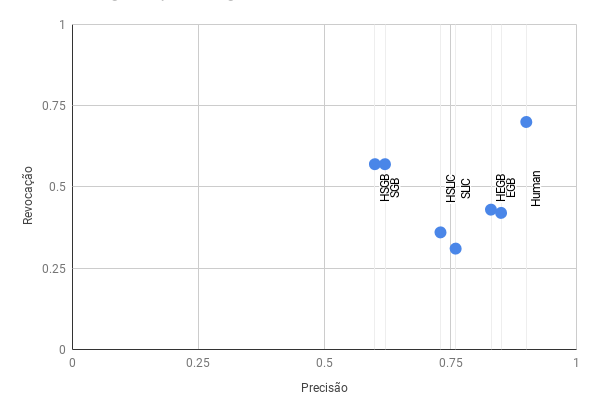
\includegraphics[width=0.95\textwidth]{graph_precision_recall.png}
\caption{Valor médio de \textit{F-measure} para os algoritmos avaliados.}
\label{gra:PREC_RECALL}
\end{figure}

\begin{figure}[ht]
\centering
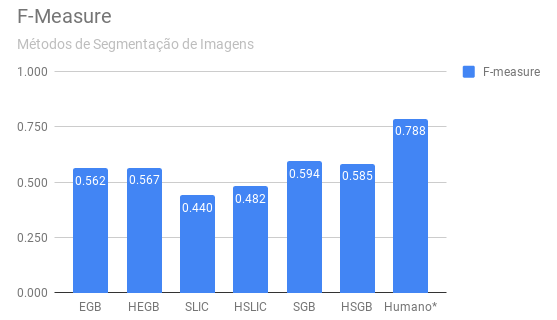
\includegraphics[width=0.95\textwidth]{graph_fmeasure.png}
\caption{Valor máximo de \textit{F-measure} para os algoritmos avaliados.}
\label{gra:FMEASURE}
\end{figure}

Conforme observamos na Figura \ref{gra:PREC_RECALL}, os algoritmos EGB e HEGB tiveram valores mais altos na métrica precisão, em relação ao algoritmo SGB e sua versão hierárquica. Entretanto, o algoritmos baseados em SGB tiveram valores superiores na métrica de revocação. Comparando ambas as métricas, por meio da \textit{F-measure}, observamos na Figura \ref{gra:FMEASURE}, que o algoritmo SGB teve valor ligeiramente superior ao algoritmo EGB. Ambos os algoritmos, e suas versões hierárquias, tiveram resultados consideravelmente superiores aos algoritmos SLIC.

As análises das Figuras \ref{gra:PREC_RECALL} e \ref{gra:FMEASURE} indicam que os algoritmos hierárquicos resultaram em valores superiores aos algoritmos sem hierarquização. Somente para o algoritmo HSGB, o resultado foi ligeiramente inferior ao obtido pelo algoritmo sem hierarquia, devido, possivelmente, ao filtro empírico de partições. Em relação a variação dos resultados, a Figura \ref{gra:THRESHOLD} mostra que a oscilação existente para os algoritmos SGB, HSGB e HEGB é consideravelmente inferior aos demais algoritmos. Esse critério indica que esses algoritmos são mais consistentes, produzindo resultados semelhantes para diferentes imagens.

\begin{figure}[ht]
\centering
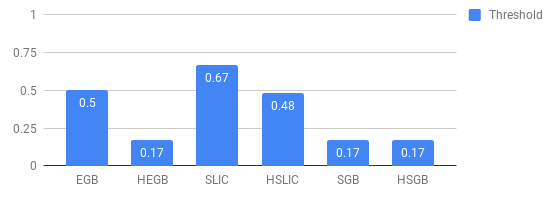
\includegraphics[width=0.9\textwidth]{graph_threshold.png}
\caption{Valor máximo de \textit{F-measure} para os algoritmos avaliados.}
\label{gra:THRESHOLD}
\end{figure}

A partir dos resultados obtidos, percebe-se que algoritmo SLIC, apesar das vantagens de produzir superpixels de tamanhos regulares, apresentou a menor eficiência para segmentação de imagens, em relação aos demais algoritmos estudados. A combinação dos algoritmos SLIC e EGB para detecção de contornos não apresentou resultado consideravelmente superior ao algoritmo EGB. Além disso, o custo de execução dos dois algoritmos em sequência e recoloração da imagens pelo pixel médio, apesar de manterem a mesma ordem de complexidade máxima $O(nlogn)$, mostraram-se injustificáveis frente ao pouco ganho obtido.

%%%%%%%%%%%%%%%%%%%%%%%%%%%%%%%%%%%%%%%%%%%%%%%%%%%%%%%
%%%%%%%%%%%%%%%%%%%%%%%%%%%%%%%%%%%%%%%%%%%%%%%%%%%%%%%

%%%%%%%%%%%%%%%%%%%%%%%%%%%%%%%%%%%%%%%%%%%%%%%%%%%%%%%
%%%%%%%%%%%%%%%%%%%%%%%%%%%%%%%%%%%%%%%%%%%%%%%%%%%%%%%
%%%%%%%%%%%%%%%%%%%%%%%%%%%%%%%%%%%%%%%%%%%%%%%%%%%%%%%

\section{Conclusão} \label{sec:conclusao}

Os algoritmos de geração de superpixels avaliados nesse trabalho tiveram resultados medianos para tarefas de segmentação e detecção de contornos, mesmo quando combinados. As versões hierárquicas dos algoritmos apresentaram resultados ligeiramente superiores àqueles obtidos sem hieraquias.

A utilização de hierarquias após a aplicação dos métodos de geração de \textit{superpixels} melhorou consideravelmente os resultados de alguns métodos. Apesar da utilização não resultar em aumento significativo da capacidade de segmentação de todos os métodos, justifica-se a utilização das versões hierárquias em relação às versões originais dos algoritmos quando houver necessidade de ampliação e redução de contornos, para efeito de agrupamento de informações. %Os parâmetros descritos nesse trabalho podem ser utilizados como passo inicial para refinamento dos parâmetros em trabalhos futuros.

Os métodos hierárquicos aqui descritos podem ser utilizados em diferentes cenários, para redução e agrupamento de segmentações de imagens, atendendo aos preceitos de análise multiescala. 

Como trabalho futuro sugere-se a utilização dos algoritmos mostrados nesse trabalho como passo de pré-processamento de outras técnicas de segmentação, como redes neurais convolucionais (\textit{convolutional neural networks}). A pré-segmentação, utilizando os métodos descritos nesse trabalho, pode permitir treinamento mais rápido das redes, ao evidenciar melhor bordas e contornos, quando houver recoloração prévia das imagens.

%%%%%%%%%%%%%%%%%%%%%%%%%%%%%%%%%%%%%%%%%%%%%%%%%%%%%%%
%%%%%%%%%%%%%%%%%%%%%%%%%%%%%%%%%%%%%%%%%%%%%%%%%%%%%%%
%%%%%%%%%%%%%%%%%%%%%%%%%%%%%%%%%%%%%%%%%%%%%%%%%%%%%%%

\bibliographystyle{sbc}
\bibliography{sbc-template}

\end{document}
